\documentclass[12pt,a4paper]{article}
\usepackage[utf8]{inputenc}
\usepackage[margin=1in]{geometry}
\usepackage{amsmath}
\usepackage{amsfonts}
\usepackage{amssymb}
\usepackage{graphicx}
\usepackage{listings}
\usepackage{xcolor}
\usepackage{fancyhdr}
\usepackage{titlesec}

% SQL syntax highlighting
\lstdefinestyle{sqlstyle}{
    language=SQL,
    basicstyle=\ttfamily\small,
    keywordstyle=\color{blue}\bfseries,
    commentstyle=\color{green!50!black},
    stringstyle=\color{red},
    numbers=left,
    numberstyle=\tiny\color{gray},
    numbersep=5pt,
    breaklines=true,
    breakatwhitespace=true,
    tabsize=2,
    showspaces=false,
    showstringspaces=false,
    frame=single,
    rulecolor=\color{gray!30},
    backgroundcolor=\color{gray!5}
}

\lstset{style=sqlstyle}

% Page setup
\pagestyle{fancy}
\fancyhf{}
\rhead{CSE 414 - Assignment 02}
\lhead{SQL practice}
\cfoot{\thepage}

% Title formatting
\titleformat{\section}{\Large\bfseries}{\thesection}{1em}{}
\titleformat{\subsection}{\large\bfseries}{\thesubsection}{1em}{}

\begin{document}

% Title Page
\begin{titlepage}
    \begin{figure}[htbp]
    \centering
    
\includegraphics[width=0.2\textwidth]{cu.png}
    \end{figure}
    \centering
    \vspace*{0.5cm}
    {\Huge\bfseries University of Chittagong}\\[0.5cm]
    {\Large Department of Computer Science \& Engineering}\\[0.5cm]
    {\large Database Systems Lab}\\[2cm]
    
    {\large Name of the assignment:}\\[0.3cm]
    {\LARGE\bfseries Chapters 5-7 Practice Problems}\\[0.5cm]
    {\large CSE 414}\\[0.5cm]
    {\large Assignment 02}\\[3cm]
    
    \begin{minipage}[t]{0.4\textwidth}
    \raggedleft
    Submitted By:\\
    \large \textbf{Debashish Chakraborty}\\
    \large ID: 23701034
    \end{minipage}
    \hspace{0.05\textwidth}
    \vrule width 1pt
    \hspace{0.05\textwidth}
    \begin{minipage}[t]{0.4\textwidth}
    Submitted To:\\
    \large \textbf{Dr. Rudra Pratap Deb Nath}\\
    \large Associate Professor
    \end{minipage}
    
    \vfill
    {\large May 31, 2025}
\end{titlepage}

\newpage
\tableofcontents
\newpage

\section{Chapter 5 Problems \& Solutions}

\subsection{Theoretical Questions}

\indent \indent \textbf{Problem 1.} Group functions work across many rows to produce one result per group.

\textbf{Solution:} TRUE

\vspace{0.5cm}

\textbf{Problem 2.} Group functions include nulls in calculations.

\textbf{Solution:} FALSE

\vspace{0.5cm}

\textbf{Problem 3.} The WHERE clause restricts rows before inclusion in a group \\\indent calculation.

\textbf{Solution:} TRUE

\vspace{0.5cm}

\subsection{Practical Problems}

\textbf{Problem 4.} Find the highest, lowest, sum, and average salary of all employees. Label the columns as Maximum, Minimum, Sum, and Average, respectively. Round your results to the nearest whole number. Save your SQL statement as lab\_05\_04.sql. Run the query.
\begin{figure}[htbp]
  \centering
  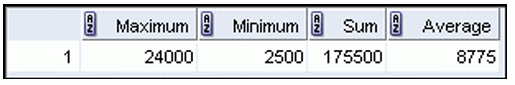
\includegraphics[width=0.6\textwidth]{Screenshots/54.png}
\end{figure}\\
\textbf{Solution:}
\begin{lstlisting}[style=sqlstyle]
SELECT 
    ROUND(MAX(SALARY)) "Maximum",
    ROUND(MIN(SALARY)) "Minimum",
    ROUND(SUM(SALARY)) "Sum",
    ROUND(AVG(SALARY)) "Average"
FROM EMPLOYEES;
\end{lstlisting}

\vspace{0.5cm}

\textbf{Problem 5.} Modify the query in lab\_05\_04.sql to display the minimum, maximum, sum, and average salary for each job type. Resave lab\_05\_04.sql as lab\_05\_05.sql. Run the statement in lab\_05\_05.sql.
\begin{figure}[htbp]
  \centering
  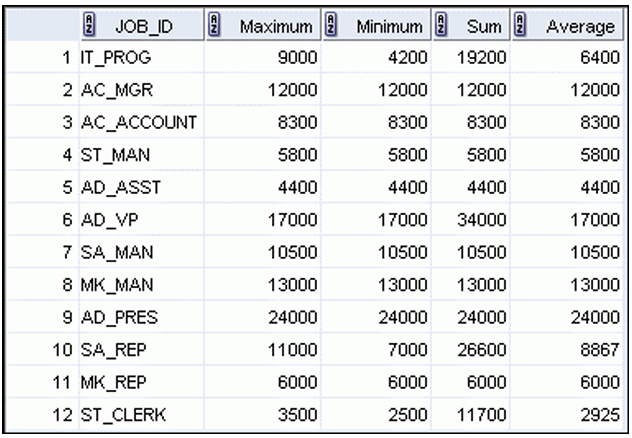
\includegraphics[width=0.4\textwidth]{Screenshots/55.png}
\end{figure}\\ \newpage
\textbf{Solution:}
\begin{lstlisting}[style=sqlstyle]
SELECT 
    JOB_ID,
    ROUND(MAX(SALARY)) "Maximum",
    ROUND(MIN(SALARY)) "Minimum",
    ROUND(SUM(SALARY)) "Sum",
    ROUND(AVG(SALARY)) "Average"
FROM EMPLOYEES
GROUP BY JOB_ID;
\end{lstlisting}

\vspace{0.5cm}

\textbf{Problem 6.} Write a query to display the number of people with the same job.
\begin{figure}[htbp]
  \centering
  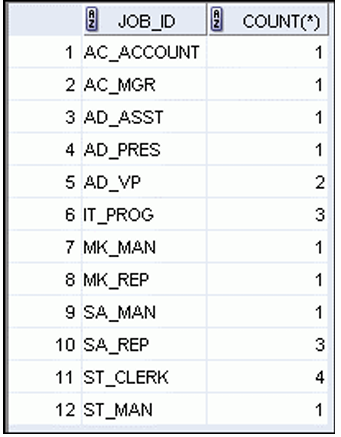
\includegraphics[width=0.3\textwidth]{Screenshots/56.png}
\end{figure}\\
\textbf{Solution:}
\begin{lstlisting}[style=sqlstyle]
SELECT 
    JOB_ID,
    COUNT(*)
FROM EMPLOYEES
GROUP BY JOB_ID;
\end{lstlisting}

Generalize the query so that the user in the HR department is prompted for a job title. Save the script to a file named lab\_05\_06.sql. Run the query. Enter IT\_PROG when prompted.
\begin{figure}[htbp]
  \centering
  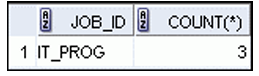
\includegraphics[width=0.4\textwidth]{Screenshots/562.png}
\end{figure}\\
\begin{lstlisting}[style=sqlstyle]
SELECT 
    JOB_ID,
    COUNT(*)
FROM EMPLOYEES
WHERE JOB_ID = UPPER('&job_id')
GROUP BY JOB_ID;
\end{lstlisting}

\vspace{0.5cm}

\textbf{Problem 7.} Determine the number of managers without listing them. Label the column as Number of Managers. Hint: Use the MANAGER\_ID column to determine the number of managers.
\begin{figure}[htbp]
  \centering
  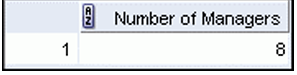
\includegraphics[width=0.4\textwidth]{Screenshots/57.png}
\end{figure}\\
\textbf{Solution:}
\begin{lstlisting}[style=sqlstyle]
SELECT COUNT(DISTINCT MANAGER_ID) "Number of Managers"
FROM EMPLOYEES;
\end{lstlisting}

\vspace{0.5cm}

\textbf{Problem 8.} Find the difference between the highest and lowest salaries. Label the column DIFFERENCE.
\begin{figure}[htbp]
  \centering
  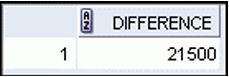
\includegraphics[width=0.3\textwidth]{Screenshots/58.png}
\end{figure}\\
\textbf{Solution:}
\begin{lstlisting}[style=sqlstyle]
SELECT MAX(SALARY) - MIN(SALARY) DIFFERENCE
FROM EMPLOYEES;
\end{lstlisting}

\vspace{0.5cm}

\textbf{Problem 9.} Create a report to display the manager number and the salary of the lowest-paid employee for that manager. Exclude anyone whose manager is not known. Exclude any groups where the minimum salary is \$6,000 or less. Sort the output in descending order of salary.
\begin{figure}[htbp]
  \centering
  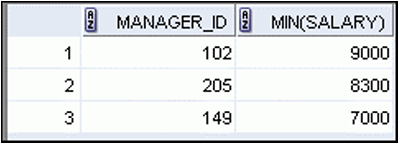
\includegraphics[width=0.4\textwidth]{Screenshots/59.png}
\end{figure}\\
\textbf{Solution:}
\begin{lstlisting}[style=sqlstyle]
SELECT 
    MANAGER_ID,
    MIN(SALARY)
FROM EMPLOYEES
WHERE MANAGER_ID IS NOT NULL
GROUP BY MANAGER_ID
HAVING MIN(SALARY) > 6000
ORDER BY MIN(SALARY) DESC;
\end{lstlisting}

\vspace{0.5cm}
\newpage
\textbf{Problem 10.} Create a query to display the total number of employees and, of that total, the number of employees hired in 1995, 1996, 1997, and 1998. Create appropriate column headings.
\begin{figure}[htbp]
  \centering
  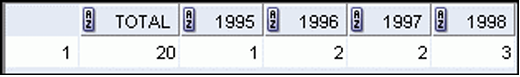
\includegraphics[width=0.6\textwidth]{Screenshots/510.png}
\end{figure}\\
\textbf{Solution:}
\begin{lstlisting}[style=sqlstyle]
SELECT COUNT(*) TOTAL,
    COUNT(DECODE(TO_CHAR(HIRE_DATE, 'YYYY'), 1995, '1')) "1995",
    COUNT(DECODE(TO_CHAR(HIRE_DATE, 'YYYY'), 1996, '1')) "1996",
    COUNT(DECODE(TO_CHAR(HIRE_DATE, 'YYYY'), 1997, '1')) "1997",
    COUNT(DECODE(TO_CHAR(HIRE_DATE, 'YYYY'), 1998, '1')) "1998"
FROM EMPLOYEES;
\end{lstlisting}

\vspace{0.5cm}

\textbf{Problem 11.} Create a matrix query to display the job, the salary for that job based on department number, and the total salary for that job, for departments 20, 50, 80, and 90, giving each column an appropriate heading.
\begin{figure}[htbp]
  \centering
  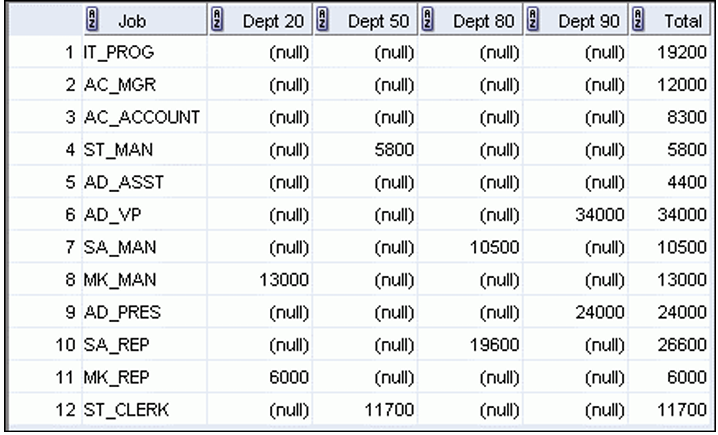
\includegraphics[width=0.7\textwidth]{Screenshots/511.png}
\end{figure}\\
\textbf{Solution:}
\begin{lstlisting}[style=sqlstyle]
SELECT DISTINCT JOB_ID "Job",
    SUM(DECODE(DEPARTMENT_ID, 20, SALARY)) "Dept 20",
    SUM(DECODE(DEPARTMENT_ID, 50, SALARY)) "Dept 50",
    SUM(DECODE(DEPARTMENT_ID, 80, SALARY)) "Dept 80",
    SUM(DECODE(DEPARTMENT_ID, 90, SALARY)) "Dept 90",
    SUM(SALARY) TOTAL
FROM EMPLOYEES
GROUP BY JOB_ID;
\end{lstlisting}

\newpage

\section{Chapter 6 Problems \& Solutions}

\textbf{Problem 1.} Write a query for the HR department to produce the addresses of all the departments. Use the LOCATIONS and COUNTRIES tables. Show the location ID, street address, city, state or province, and country in the output. Use a NATURAL JOIN to produce the results.
\begin{figure}[htbp]
  \centering
  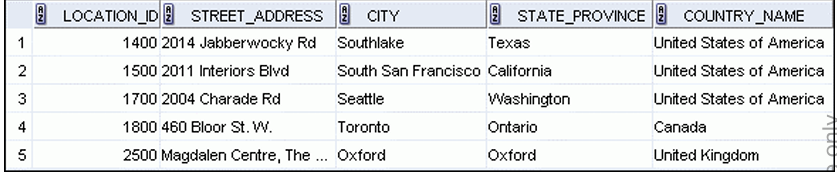
\includegraphics[width=0.8\textwidth]{Screenshots/61.png}
\end{figure}\\
\textbf{Solution:}
\begin{lstlisting}[style=sqlstyle]
SELECT 
    LOCATION_ID,
    STREET_ADDRESS,
    CITY,
    STATE_PROVINCE,
    COUNTRY_NAME
FROM LOCATIONS
NATURAL JOIN COUNTRIES;
\end{lstlisting}

\vspace{0.5cm}

\textbf{Problem 2.} The HR department needs a report of all employees. Write a query to display the last name, department number, and department name for all the employees.
\begin{figure}[htbp]
  \centering
  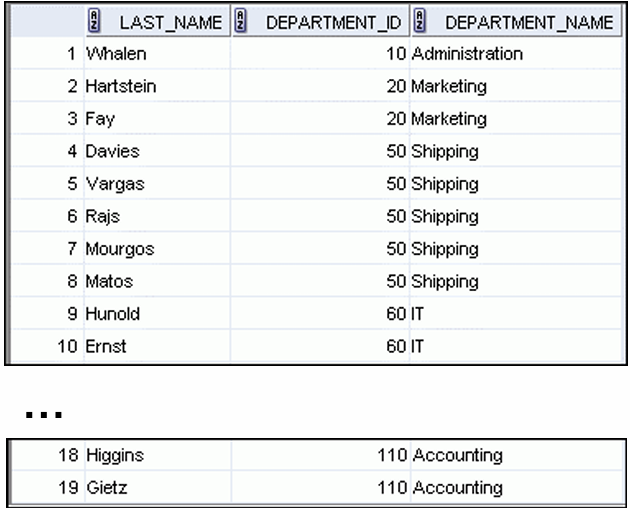
\includegraphics[width=0.5\textwidth]{Screenshots/62.png}
\end{figure}\\
\textbf{Solution:}
\begin{lstlisting}[style=sqlstyle]
SELECT 
    LAST_NAME,
    DEPARTMENT_ID,
    DEPARTMENT_NAME
FROM EMPLOYEES
JOIN DEPARTMENTS USING (DEPARTMENT_ID);
\end{lstlisting}

\vspace{0.5cm}

\textbf{Problem 3.} The HR department needs a report of employees in Toronto. Display the last name, job, department number, and the department name for all employees who work in Toronto.
\begin{figure}[htbp]
  \centering
  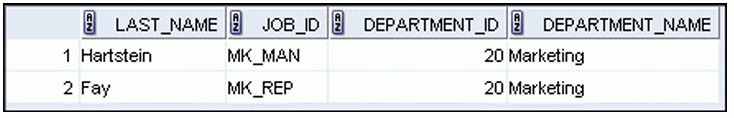
\includegraphics[width=0.7\textwidth]{Screenshots/63.png}
\end{figure}\\
\textbf{Solution:}
\begin{lstlisting}[style=sqlstyle]
SELECT 
    LAST_NAME,
    JOB_ID,
    DEPARTMENT_ID,
    DEPARTMENT_NAME
FROM EMPLOYEES
JOIN DEPARTMENTS USING (DEPARTMENT_ID)
JOIN LOCATIONS USING (LOCATION_ID)
WHERE CITY = 'Toronto';
\end{lstlisting}

\vspace{0.5cm}

\textbf{Problem 4.} Create a report to display employees' last name and employee number along with their manager's last name and manager number. Label the columns Employee, Emp\#, Manager, and Mgr\#, respectively. Save your SQL statement as lab\_06\_04.sql. Run the query.
\begin{figure}[htbp]
  \centering
  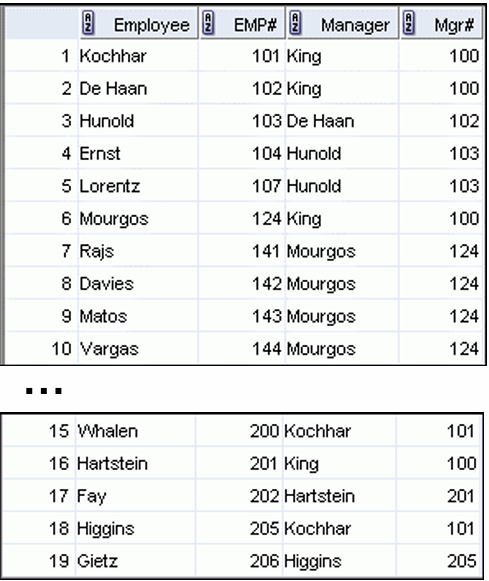
\includegraphics[width=0.4\textwidth]{Screenshots/64.png}
\end{figure}
\textbf{Solution:}
\begin{lstlisting}[style=sqlstyle]
SELECT 
    E.LAST_NAME "Employee",
    E.EMPLOYEE_ID "Emp#",
    M.LAST_NAME "Manager",
    M.EMPLOYEE_ID "Mgr#"
FROM EMPLOYEES E
JOIN EMPLOYEES M ON (E.MANAGER_ID = M.EMPLOYEE_ID)
ORDER BY E.EMPLOYEE_ID;
\end{lstlisting}

\vspace{0.5cm}

\textbf{Problem 5.} Modify lab\_06\_04.sql to display all employees including King, who has no manager. Order the results by the employee number. Save your SQL statement as lab\_06\_05.sql. Run the query in lab\_06\_05.sql.
\begin{figure}[htbp]
  \centering
  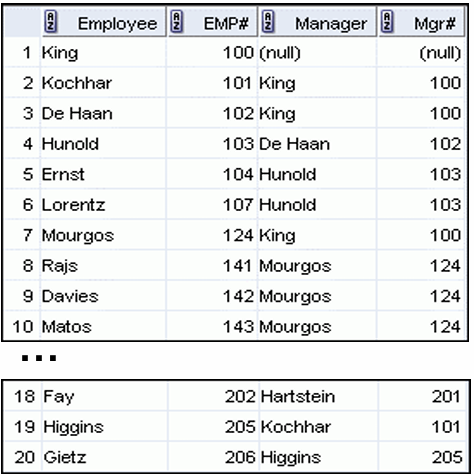
\includegraphics[width=0.5\textwidth]{Screenshots/65.png}
\end{figure}\\
\textbf{Solution:}
\begin{lstlisting}[style=sqlstyle]
SELECT 
    E.LAST_NAME "Employee",
    E.EMPLOYEE_ID "Emp#",
    M.LAST_NAME "Manager",
    M.EMPLOYEE_ID "Mgr#"
FROM EMPLOYEES E
LEFT JOIN EMPLOYEES M ON (E.MANAGER_ID = M.EMPLOYEE_ID)
ORDER BY E.EMPLOYEE_ID;
\end{lstlisting}

\vspace{0.5cm}

\textbf{Problem 6.} Create a report for the HR department that displays employee last names, department numbers, and all the employees who work in the same department as a given employee. Give each column an appropriate label. Save the script to a file named lab\_06\_06.sql.
\begin{figure}[htbp]
  \centering
  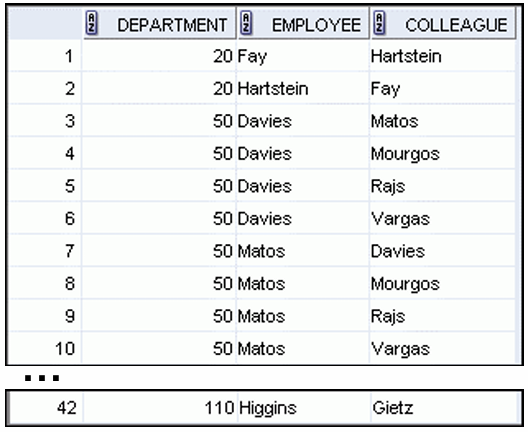
\includegraphics[width=0.4\textwidth]{Screenshots/66.png}
\end{figure}\newpage
\textbf{Solution:}
\begin{lstlisting}[style=sqlstyle]
SELECT 
    E.DEPARTMENT_ID DEPARTMENT,
    E.LAST_NAME EMPLOYEE,
    C.LAST_NAME COLLEAGUE
FROM EMPLOYEES E
JOIN EMPLOYEES C ON (E.DEPARTMENT_ID = C.DEPARTMENT_ID)
WHERE E.EMPLOYEE_ID <> C.EMPLOYEE_ID
ORDER BY DEPARTMENT, EMPLOYEE, COLLEAGUE;
\end{lstlisting}

\vspace{0.5cm}

\textbf{Problem 7.} The HR department needs a report on job grades and salaries. To familiarize yourself with the JOB\_GRADES table, first show the structure of the JOB\_GRADES table. Then create a query that displays the name, job, department name, salary, and grade for all employees.
\begin{figure}[htbp]
  \centering
  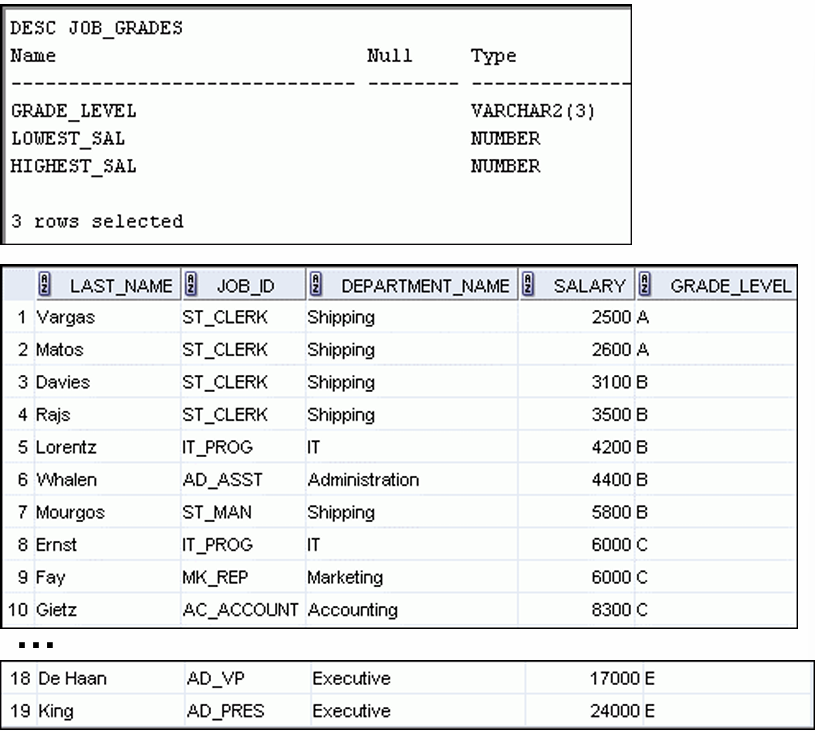
\includegraphics[width=0.6\textwidth]{Screenshots/67.png}
\end{figure}\\
\textbf{Solution:}
\begin{lstlisting}[style=sqlstyle]
SELECT 
    LAST_NAME,
    JOB_ID,
    DEPARTMENT_NAME,
    SALARY,
    GRADE_LEVEL
FROM EMPLOYEES
JOIN DEPARTMENTS USING (DEPARTMENT_ID)
JOIN JOB_GRADES ON (SALARY BETWEEN LOWEST_SAL AND HIGHEST_SAL)
ORDER BY SALARY;
\end{lstlisting}

\vspace{0.5cm}
\newpage
\textbf{Problem 8.} The HR department wants to determine the names of all the employees who were hired after Davies. Create a query to display the name and hire date of any employee hired after employee Davies.
\begin{figure}[htbp]
  \centering
  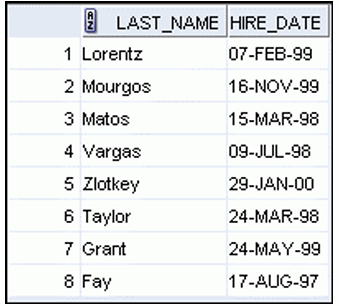
\includegraphics[width=0.4\textwidth]{Screenshots/68.png}
\end{figure}\\
\textbf{Solution:}
\begin{lstlisting}[style=sqlstyle]
SELECT 
    E.LAST_NAME,
    TO_CHAR(E.HIRE_DATE, 'DD-MON-YY') HIRE_DATE
FROM EMPLOYEES E
JOIN EMPLOYEES DAVIES ON (DAVIES.LAST_NAME = 'Davies')
WHERE DAVIES.HIRE_DATE < E.HIRE_DATE;
\end{lstlisting}

\vspace{0.5cm}

\textbf{Problem 9.} The HR department needs to find the names and hire dates of all the employees who were hired before their managers, along with their managers' names and hire dates. Save the script to a file named lab\_06\_09.sql.
\begin{figure}[htbp]
  \centering
  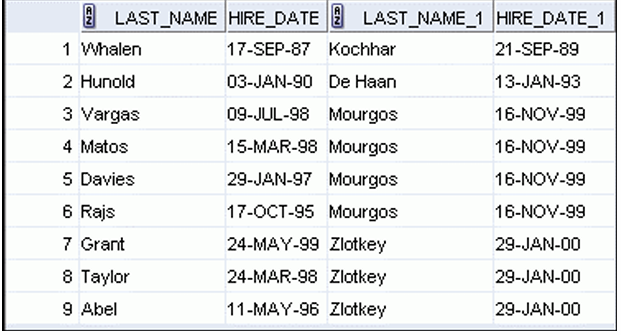
\includegraphics[width=0.5\textwidth]{Screenshots/69.png}
\end{figure}\\
\textbf{Solution:}
\begin{lstlisting}[style=sqlstyle]
SELECT 
    E.LAST_NAME,
    TO_CHAR(E.HIRE_DATE, 'DD-MON-YY') HIRE_DATE,
    M.LAST_NAME,
    TO_CHAR(M.HIRE_DATE, 'DD-MON-YY') HIRE_DATE1
FROM EMPLOYEES E
JOIN EMPLOYEES M ON (E.MANAGER_ID = M.EMPLOYEE_ID)
WHERE E.HIRE_DATE < M.HIRE_DATE;
\end{lstlisting}

\newpage

\section{Chapter 7 Problems \& Solutions}

\textbf{Problem 1.} The HR department needs a query that prompts the user for an employee last name. The query then displays the last name and hire date of any employee in the same department as the employee whose name they supply (excluding that employee). For example, if the user enters Zlotkey, find all employees who work with Zlotkey (excluding Zlotkey).
\begin{figure}[htbp]
  \centering
  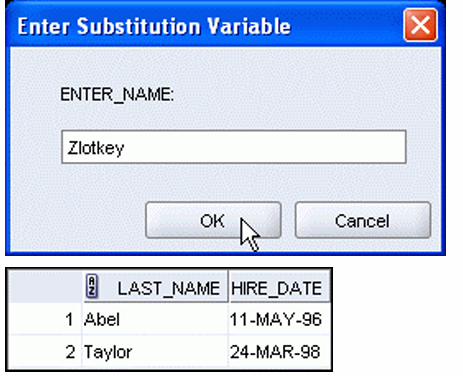
\includegraphics[width=0.4\textwidth]{Screenshots/71.png}
\end{figure}\\
\textbf{Solution:}
\begin{lstlisting}[style=sqlstyle]
SELECT 
    LAST_NAME,
    TO_CHAR(HIRE_DATE, 'DD-MON-YY') HIRE_DATE
FROM EMPLOYEES
WHERE DEPARTMENT_ID = (
    SELECT DEPARTMENT_ID
    FROM EMPLOYEES
    WHERE LAST_NAME = INITCAP('&&last_name')
)
AND LAST_NAME <> INITCAP('&&last_name');
\end{lstlisting}

\vspace{0.5cm}

\textbf{Problem 2.} Create a report that displays the employee number, last name, and salary of all employees who earn more than the average salary. Sort the results in order of ascending salary.
\begin{figure}[htbp]
  \centering
  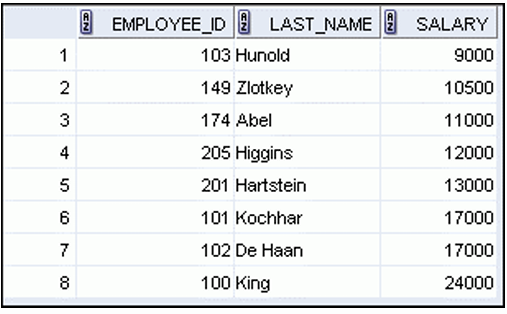
\includegraphics[width=0.5\textwidth]{Screenshots/72.png}
\end{figure}\\
\newpage
\textbf{Solution:}
\begin{lstlisting}[style=sqlstyle]
SELECT 
    EMPLOYEE_ID,
    LAST_NAME,
    SALARY
FROM EMPLOYEES
WHERE SALARY > (
    SELECT AVG(SALARY)
    FROM EMPLOYEES
)
ORDER BY SALARY;
\end{lstlisting}

\vspace{0.5cm}

\textbf{Problem 3.} Write a query that displays the employee number and last name of all employees who work in a department with any employee whose last name contains the letter "u." Save your SQL statement as lab\_07\_03.sql. Run your query.
\begin{figure}[htbp]
  \centering
  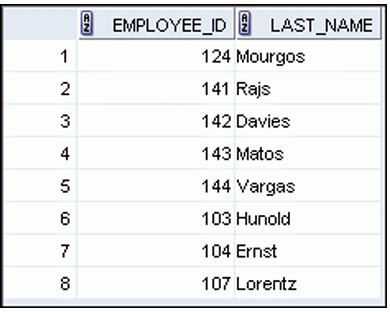
\includegraphics[width=0.5\textwidth]{Screenshots/73.png}
\end{figure}\\
\textbf{Solution:}
\begin{lstlisting}[style=sqlstyle]
SELECT 
    EMPLOYEE_ID,
    LAST_NAME
FROM EMPLOYEES
WHERE DEPARTMENT_ID IN (
    SELECT DEPARTMENT_ID
    FROM EMPLOYEES
    WHERE LAST_NAME LIKE '%u%'
);
\end{lstlisting}

\vspace{0.5cm}
\newpage
\textbf{Problem 4.} The HR department needs a report that displays the last name, department number, and job ID of all employees whose department location ID is 1700.
\begin{figure}[htbp]
  \centering
  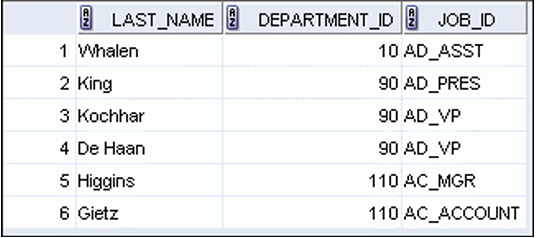
\includegraphics[width=0.5\textwidth]{Screenshots/74.png}
\end{figure}\\
\textbf{Solution:}
\begin{lstlisting}[style=sqlstyle]
SELECT 
    LAST_NAME,
    DEPARTMENT_ID,
    JOB_ID
FROM EMPLOYEES
WHERE DEPARTMENT_ID IN (
    SELECT DEPARTMENT_ID
    FROM DEPARTMENTS
    WHERE LOCATION_ID = 1700
)
ORDER BY DEPARTMENT_ID;
\end{lstlisting}

Modify the query so that the user is prompted for a location ID. Save this to a file named lab\_07\_04.sql.

\begin{lstlisting}[style=sqlstyle]
SELECT 
    LAST_NAME,
    DEPARTMENT_ID,
    JOB_ID
FROM EMPLOYEES
WHERE DEPARTMENT_ID IN (
    SELECT DEPARTMENT_ID
    FROM DEPARTMENTS
    WHERE LOCATION_ID = &LOCATION_ID
)
ORDER BY DEPARTMENT_ID;
\end{lstlisting}

\vspace{0.5cm}

\textbf{Problem 5.} Create a report for HR that displays the last name and salary of every employee who reports to King.
\begin{figure}[htbp]
  \centering
  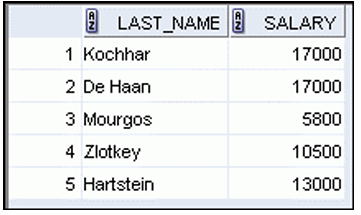
\includegraphics[width=0.4\textwidth]{Screenshots/75.png}
\end{figure}\\
\textbf{Solution:}
\begin{lstlisting}[style=sqlstyle]
SELECT 
    LAST_NAME,
    SALARY
FROM EMPLOYEES
WHERE MANAGER_ID = (
    SELECT EMPLOYEE_ID
    FROM EMPLOYEES
    WHERE LAST_NAME = 'King'
);
\end{lstlisting}

\vspace{0.5cm}

\textbf{Problem 6.} Create a report for HR that displays the department number, last name, and job ID for every employee in the Executive department.
\begin{figure}[htbp]
  \centering
  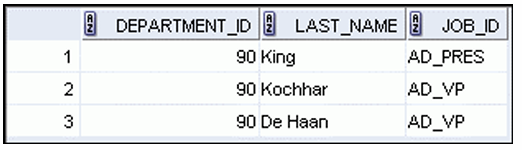
\includegraphics[width=0.5\textwidth]{Screenshots/76.png}
\end{figure}\\
\textbf{Solution:}
\begin{lstlisting}[style=sqlstyle]
SELECT 
    DEPARTMENT_ID,
    LAST_NAME,
    JOB_ID
FROM EMPLOYEES
WHERE DEPARTMENT_ID = (
    SELECT DEPARTMENT_ID
    FROM DEPARTMENTS
    WHERE DEPARTMENT_NAME = 'Executive'
);
\end{lstlisting}

\vspace{0.5cm}

\textbf{Problem 7.} Modify the query in lab\_07\_03.sql to display the employee number, last name, and salary of all employees who earn more than the average salary, and who work in a department with any employee whose last name contains a "u." Resave lab\_07\_03.sql as lab\_07\_07.sql. Run the statement in lab\_07\_07.sql.
\begin{figure}[htbp]
  \centering
  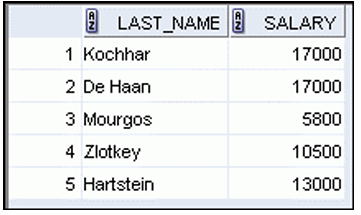
\includegraphics[width=0.4\textwidth]{Screenshots/75.png}
\end{figure}\\
\newpage
\textbf{Solution:}
\begin{lstlisting}[style=sqlstyle]
SELECT 
    EMPLOYEE_ID,
    LAST_NAME,
    SALARY
FROM EMPLOYEES
WHERE SALARY > (
    SELECT AVG(SALARY)
    FROM EMPLOYEES
)
AND DEPARTMENT_ID IN (
    SELECT DEPARTMENT_ID
    FROM EMPLOYEES
    WHERE LAST_NAME LIKE '%u%'
);
\end{lstlisting}

\end{document}